\documentclass{jsarticle}
\usepackage[dvipdfmx]{graphicx}
\usepackage{amsmath,amssymb}

\newcommand{\argmax}{\mathop{\rm arg~max}\limits}
\newcommand{\argmin}{\mathop{\rm arg~min}\limits}

\begin{document}

\title{ Matrix Profile XII: MPdist \\(An Ultra-Fast Time Series Distance Measure to
	allow Data Mining in more Complex Real-World
	Deployments)}
\author{著者:Shaghayegh Gharghabi, Shima Imani, Anthony Bagnall2
	,\\ Amirali Darvishzadeh, Eamonn Keogh
}
\date{}
\maketitle
会議名,年: IEEE International Conference on Data Mining, 2018, pp. 17–20.

\section{概要}
\subsection{どんな論文?}
2つの時系列に似たような部分時系列が含まれていれば距離が小さくなるような、新しい距離尺度(MPdist)を提案(計算にはMatrix Profileを用いる).
\subsection{比較対象}
\begin{itemize}
	\item ユークリッド距離
	\item DTW
\end{itemize}

\subsection{メリット}
\begin{itemize}
	\item 時系列の長さが違っても測定可能
	\item ベースラインの異なる時系列やspike等に対してロバスト
	\begin{figure}[h!]
		\begin{center}
			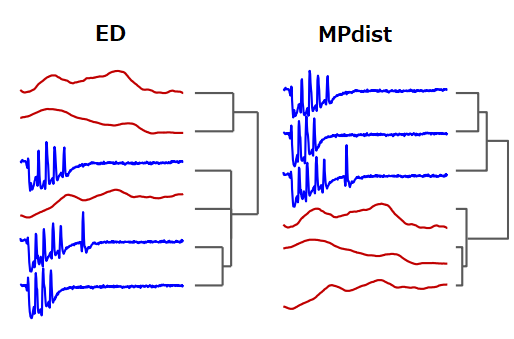
\includegraphics[scale = 0.5]{MPdist_fig2.png}
		\end{center}
		\caption{ユークリッド距離とMPdistを用いて階層的クラスタリング(最長距離法)を行った結果}
%		\label{fig:sleep_example}
	\end{figure}
\end{itemize}

\subsection{MPdistの計算}
\begin{enumerate}
	\item 時系列$\boldsymbol{A}$と$\boldsymbol{B}$のMatrix Profileである$\mathrm{MP}_{\boldsymbol{AB}}$と$\mathrm{MP}_{\boldsymbol{BA}}$を計算\\
	\item $\mathrm{MP}_{\boldsymbol{AB}}$と$\mathrm{MP}_{\boldsymbol{BA}}$のうち,$k$番目に小さい値がMPdistとなる(論文中では$k = 2 \times \mathrm{len(A)} \times \mathrm{len(B)} \times 0.05$を使っている)
\end{enumerate}


\subsection{MPdistベクトル}
長さ$n$の時系列$\boldsymbol{Q}$と,それよりも長い長さ$m$の時系列$\boldsymbol{T}$が与えられたとき,$\boldsymbol{Q}$と$\boldsymbol{T}_{i,n}$のMPdistを$i=1~m-n-1$の範囲全てで求めたものをMPdistベクトルと呼ぶ($\boldsymbol{T}_{i,n}$はインデックス$i$で始まる長さ$n$の部分時系列).式で書くと以下で表せる.
\begin{displaymath}
\mathrm{MPdistvec}_i = \mathrm{MPdist}(\boldsymbol{Q},\boldsymbol{T}_{i,n})
\end{displaymath}
普通に計算(matrix profileは高速化していると仮定)すると$O(n^2m)$だが,高速化により$O(nm)$で計算できる.

\subsection{感想・メモ}
\begin{itemize}
	\item ユークリッド距離やDTW距離みたいに時系列全体を使って距離を計算すると,ノイズや振幅方向の歪みに敏感になってしまうので,部分時系列を比較することは有意義と感じた.
	\item 長さ$n$と$m$の時系列のMPdistの計算量は$O(nm)$なので,長い時系列に適用するには工夫が必要.
	\item MPdistベクトルはSnippetsを求める際に用いられる.
\end{itemize}
\end{document}